\section{Organisationsplan för hela projektet}
Beställaren har beställt projektet från gruppen. Projektledaren är den medlem i gruppen som agerar mellanhand mellan projektgruppen och beställaren. Varje medlem i projektgruppen har ett ansvarsområde där han eller hon leder en arbetsgrupp bestående av delar av resten av gruppen. Det innebär att varje medlem är både arbetsledare och del i minst ett annat arbetslag. En handledare och en grupp tekniska experter finns tillgängliga om gruppen behöver hjälp att lösa något specifikt problem. Figur \ref{projektplan:organisationsplan} illustrerar strukturen.

\begin{figure}[h!]
\center
\tikzset{every picture/.style={scale=0.6}}%
% Graphic for TeX using PGF
% Title: /home/hannes/GitHub/TSEA29/dokumentation/projektplan/projektplan-organisationsplan.dia
% Creator: Dia v0.97.2
% CreationDate: Thu Sep 25 17:08:40 2014
% For: hannes
% \usepackage{tikz}
% The following commands are not supported in PSTricks at present
% We define them conditionally, so when they are implemented,
% this pgf file will use them.
\ifx\du\undefined
  \newlength{\du}
\fi
\setlength{\du}{15\unitlength}
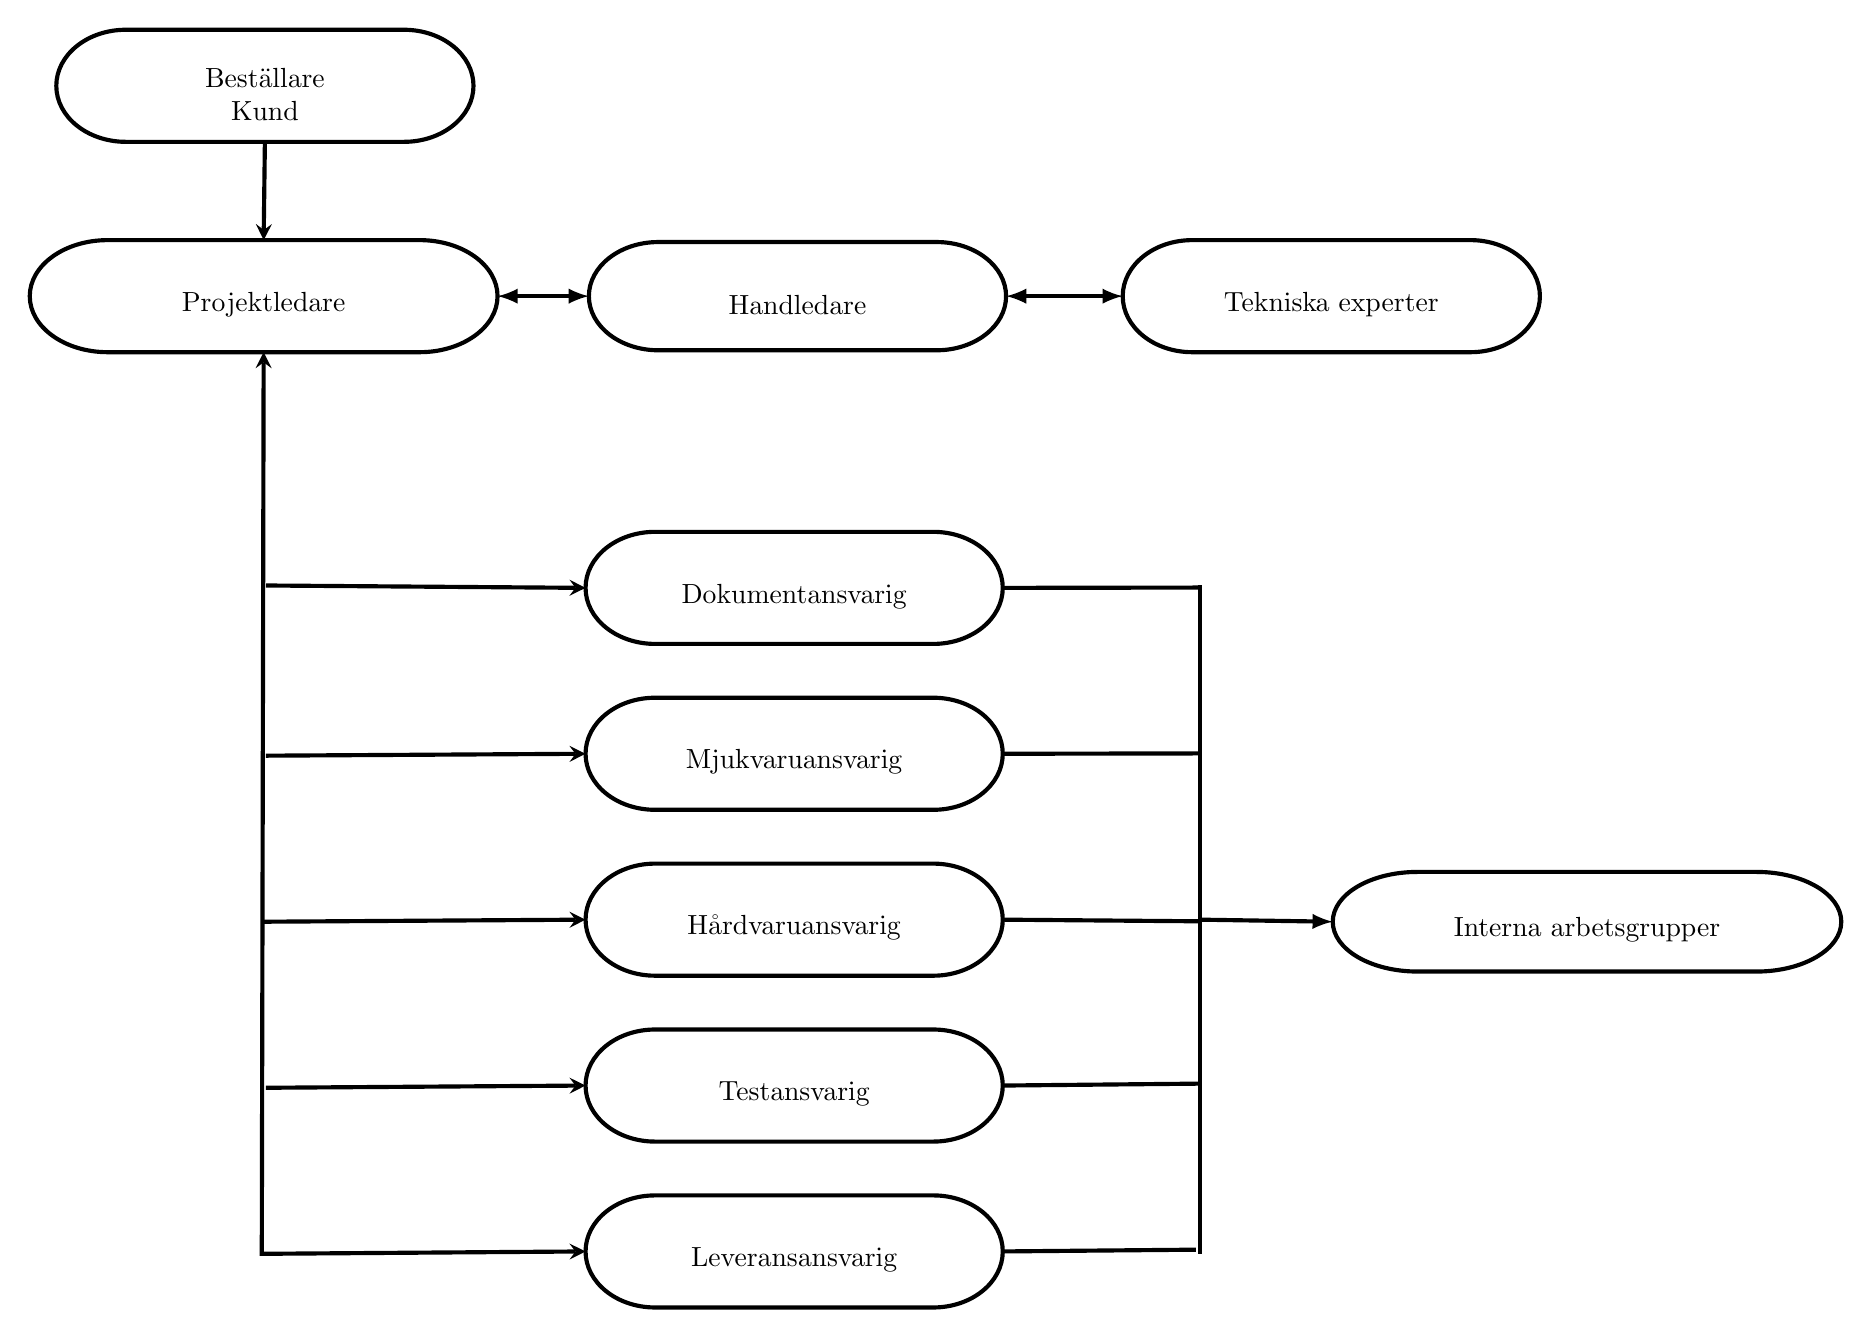
\begin{tikzpicture}
\pgftransformxscale{1.000000}
\pgftransformyscale{-1.000000}
\definecolor{dialinecolor}{rgb}{0.000000, 0.000000, 0.000000}
\pgfsetstrokecolor{dialinecolor}
\definecolor{dialinecolor}{rgb}{1.000000, 1.000000, 1.000000}
\pgfsetfillcolor{dialinecolor}
\pgfsetlinewidth{0.100000\du}
\pgfsetdash{}{0pt}
\pgfsetdash{}{0pt}
\pgfsetbuttcap
\pgfsetmiterjoin
\pgfsetlinewidth{0.100000\du}
\pgfsetbuttcap
\pgfsetmiterjoin
\pgfsetdash{}{0pt}
\definecolor{dialinecolor}{rgb}{1.000000, 1.000000, 1.000000}
\pgfsetfillcolor{dialinecolor}
\pgfpathmoveto{\pgfpoint{17.075000\du}{8.950000\du}}
\pgfpathlineto{\pgfpoint{23.775000\du}{8.950000\du}}
\pgfpathcurveto{\pgfpoint{24.700077\du}{8.950000\du}}{\pgfpoint{25.450000\du}{9.554415\du}}{\pgfpoint{25.450000\du}{10.300000\du}}
\pgfpathcurveto{\pgfpoint{25.450000\du}{11.045585\du}}{\pgfpoint{24.700077\du}{11.650000\du}}{\pgfpoint{23.775000\du}{11.650000\du}}
\pgfpathlineto{\pgfpoint{17.075000\du}{11.650000\du}}
\pgfpathcurveto{\pgfpoint{16.149923\du}{11.650000\du}}{\pgfpoint{15.400000\du}{11.045585\du}}{\pgfpoint{15.400000\du}{10.300000\du}}
\pgfpathcurveto{\pgfpoint{15.400000\du}{9.554415\du}}{\pgfpoint{16.149923\du}{8.950000\du}}{\pgfpoint{17.075000\du}{8.950000\du}}
\pgfusepath{fill}
\definecolor{dialinecolor}{rgb}{0.000000, 0.000000, 0.000000}
\pgfsetstrokecolor{dialinecolor}
\pgfpathmoveto{\pgfpoint{17.075000\du}{8.950000\du}}
\pgfpathlineto{\pgfpoint{23.775000\du}{8.950000\du}}
\pgfpathcurveto{\pgfpoint{24.700077\du}{8.950000\du}}{\pgfpoint{25.450000\du}{9.554415\du}}{\pgfpoint{25.450000\du}{10.300000\du}}
\pgfpathcurveto{\pgfpoint{25.450000\du}{11.045585\du}}{\pgfpoint{24.700077\du}{11.650000\du}}{\pgfpoint{23.775000\du}{11.650000\du}}
\pgfpathlineto{\pgfpoint{17.075000\du}{11.650000\du}}
\pgfpathcurveto{\pgfpoint{16.149923\du}{11.650000\du}}{\pgfpoint{15.400000\du}{11.045585\du}}{\pgfpoint{15.400000\du}{10.300000\du}}
\pgfpathcurveto{\pgfpoint{15.400000\du}{9.554415\du}}{\pgfpoint{16.149923\du}{8.950000\du}}{\pgfpoint{17.075000\du}{8.950000\du}}
\pgfusepath{stroke}
% setfont left to latex
\definecolor{dialinecolor}{rgb}{0.000000, 0.000000, 0.000000}
\pgfsetstrokecolor{dialinecolor}
\node at (20.425000\du,10.100000\du){Beställare};
% setfont left to latex
\definecolor{dialinecolor}{rgb}{0.000000, 0.000000, 0.000000}
\pgfsetstrokecolor{dialinecolor}
\node at (20.425000\du,10.900000\du){Kund};
\pgfsetlinewidth{0.100000\du}
\pgfsetdash{}{0pt}
\pgfsetdash{}{0pt}
\pgfsetbuttcap
\pgfsetmiterjoin
\pgfsetlinewidth{0.100000\du}
\pgfsetbuttcap
\pgfsetmiterjoin
\pgfsetdash{}{0pt}
\definecolor{dialinecolor}{rgb}{1.000000, 1.000000, 1.000000}
\pgfsetfillcolor{dialinecolor}
\pgfpathmoveto{\pgfpoint{16.638750\du}{14.017500\du}}
\pgfpathlineto{\pgfpoint{24.151250\du}{14.017500\du}}
\pgfpathcurveto{\pgfpoint{25.188510\du}{14.017500\du}}{\pgfpoint{26.029375\du}{14.621915\du}}{\pgfpoint{26.029375\du}{15.367500\du}}
\pgfpathcurveto{\pgfpoint{26.029375\du}{16.113085\du}}{\pgfpoint{25.188510\du}{16.717500\du}}{\pgfpoint{24.151250\du}{16.717500\du}}
\pgfpathlineto{\pgfpoint{16.638750\du}{16.717500\du}}
\pgfpathcurveto{\pgfpoint{15.601490\du}{16.717500\du}}{\pgfpoint{14.760625\du}{16.113085\du}}{\pgfpoint{14.760625\du}{15.367500\du}}
\pgfpathcurveto{\pgfpoint{14.760625\du}{14.621915\du}}{\pgfpoint{15.601490\du}{14.017500\du}}{\pgfpoint{16.638750\du}{14.017500\du}}
\pgfusepath{fill}
\definecolor{dialinecolor}{rgb}{0.000000, 0.000000, 0.000000}
\pgfsetstrokecolor{dialinecolor}
\pgfpathmoveto{\pgfpoint{16.638750\du}{14.017500\du}}
\pgfpathlineto{\pgfpoint{24.151250\du}{14.017500\du}}
\pgfpathcurveto{\pgfpoint{25.188510\du}{14.017500\du}}{\pgfpoint{26.029375\du}{14.621915\du}}{\pgfpoint{26.029375\du}{15.367500\du}}
\pgfpathcurveto{\pgfpoint{26.029375\du}{16.113085\du}}{\pgfpoint{25.188510\du}{16.717500\du}}{\pgfpoint{24.151250\du}{16.717500\du}}
\pgfpathlineto{\pgfpoint{16.638750\du}{16.717500\du}}
\pgfpathcurveto{\pgfpoint{15.601490\du}{16.717500\du}}{\pgfpoint{14.760625\du}{16.113085\du}}{\pgfpoint{14.760625\du}{15.367500\du}}
\pgfpathcurveto{\pgfpoint{14.760625\du}{14.621915\du}}{\pgfpoint{15.601490\du}{14.017500\du}}{\pgfpoint{16.638750\du}{14.017500\du}}
\pgfusepath{stroke}
% setfont left to latex
\definecolor{dialinecolor}{rgb}{0.000000, 0.000000, 0.000000}
\pgfsetstrokecolor{dialinecolor}
\node at (20.395000\du,15.567500\du){Projektledare};
\pgfsetlinewidth{0.100000\du}
\pgfsetdash{}{0pt}
\pgfsetdash{}{0pt}
\pgfsetbuttcap
\pgfsetmiterjoin
\pgfsetlinewidth{0.100000\du}
\pgfsetbuttcap
\pgfsetmiterjoin
\pgfsetdash{}{0pt}
\definecolor{dialinecolor}{rgb}{1.000000, 1.000000, 1.000000}
\pgfsetfillcolor{dialinecolor}
\pgfpathmoveto{\pgfpoint{29.905000\du}{14.063750\du}}
\pgfpathlineto{\pgfpoint{36.605000\du}{14.063750\du}}
\pgfpathcurveto{\pgfpoint{37.530077\du}{14.063750\du}}{\pgfpoint{38.280000\du}{14.647458\du}}{\pgfpoint{38.280000\du}{15.367500\du}}
\pgfpathcurveto{\pgfpoint{38.280000\du}{16.087542\du}}{\pgfpoint{37.530077\du}{16.671250\du}}{\pgfpoint{36.605000\du}{16.671250\du}}
\pgfpathlineto{\pgfpoint{29.905000\du}{16.671250\du}}
\pgfpathcurveto{\pgfpoint{28.979923\du}{16.671250\du}}{\pgfpoint{28.230000\du}{16.087542\du}}{\pgfpoint{28.230000\du}{15.367500\du}}
\pgfpathcurveto{\pgfpoint{28.230000\du}{14.647458\du}}{\pgfpoint{28.979923\du}{14.063750\du}}{\pgfpoint{29.905000\du}{14.063750\du}}
\pgfusepath{fill}
\definecolor{dialinecolor}{rgb}{0.000000, 0.000000, 0.000000}
\pgfsetstrokecolor{dialinecolor}
\pgfpathmoveto{\pgfpoint{29.905000\du}{14.063750\du}}
\pgfpathlineto{\pgfpoint{36.605000\du}{14.063750\du}}
\pgfpathcurveto{\pgfpoint{37.530077\du}{14.063750\du}}{\pgfpoint{38.280000\du}{14.647458\du}}{\pgfpoint{38.280000\du}{15.367500\du}}
\pgfpathcurveto{\pgfpoint{38.280000\du}{16.087542\du}}{\pgfpoint{37.530077\du}{16.671250\du}}{\pgfpoint{36.605000\du}{16.671250\du}}
\pgfpathlineto{\pgfpoint{29.905000\du}{16.671250\du}}
\pgfpathcurveto{\pgfpoint{28.979923\du}{16.671250\du}}{\pgfpoint{28.230000\du}{16.087542\du}}{\pgfpoint{28.230000\du}{15.367500\du}}
\pgfpathcurveto{\pgfpoint{28.230000\du}{14.647458\du}}{\pgfpoint{28.979923\du}{14.063750\du}}{\pgfpoint{29.905000\du}{14.063750\du}}
\pgfusepath{stroke}
% setfont left to latex
\definecolor{dialinecolor}{rgb}{0.000000, 0.000000, 0.000000}
\pgfsetstrokecolor{dialinecolor}
\node at (33.255000\du,15.567500\du){Handledare};
\pgfsetlinewidth{0.100000\du}
\pgfsetdash{}{0pt}
\pgfsetdash{}{0pt}
\pgfsetbuttcap
\pgfsetmiterjoin
\pgfsetlinewidth{0.100000\du}
\pgfsetbuttcap
\pgfsetmiterjoin
\pgfsetdash{}{0pt}
\definecolor{dialinecolor}{rgb}{1.000000, 1.000000, 1.000000}
\pgfsetfillcolor{dialinecolor}
\pgfpathmoveto{\pgfpoint{42.765000\du}{14.017500\du}}
\pgfpathlineto{\pgfpoint{49.465000\du}{14.017500\du}}
\pgfpathcurveto{\pgfpoint{50.390077\du}{14.017500\du}}{\pgfpoint{51.140000\du}{14.621915\du}}{\pgfpoint{51.140000\du}{15.367500\du}}
\pgfpathcurveto{\pgfpoint{51.140000\du}{16.113085\du}}{\pgfpoint{50.390077\du}{16.717500\du}}{\pgfpoint{49.465000\du}{16.717500\du}}
\pgfpathlineto{\pgfpoint{42.765000\du}{16.717500\du}}
\pgfpathcurveto{\pgfpoint{41.839923\du}{16.717500\du}}{\pgfpoint{41.090000\du}{16.113085\du}}{\pgfpoint{41.090000\du}{15.367500\du}}
\pgfpathcurveto{\pgfpoint{41.090000\du}{14.621915\du}}{\pgfpoint{41.839923\du}{14.017500\du}}{\pgfpoint{42.765000\du}{14.017500\du}}
\pgfusepath{fill}
\definecolor{dialinecolor}{rgb}{0.000000, 0.000000, 0.000000}
\pgfsetstrokecolor{dialinecolor}
\pgfpathmoveto{\pgfpoint{42.765000\du}{14.017500\du}}
\pgfpathlineto{\pgfpoint{49.465000\du}{14.017500\du}}
\pgfpathcurveto{\pgfpoint{50.390077\du}{14.017500\du}}{\pgfpoint{51.140000\du}{14.621915\du}}{\pgfpoint{51.140000\du}{15.367500\du}}
\pgfpathcurveto{\pgfpoint{51.140000\du}{16.113085\du}}{\pgfpoint{50.390077\du}{16.717500\du}}{\pgfpoint{49.465000\du}{16.717500\du}}
\pgfpathlineto{\pgfpoint{42.765000\du}{16.717500\du}}
\pgfpathcurveto{\pgfpoint{41.839923\du}{16.717500\du}}{\pgfpoint{41.090000\du}{16.113085\du}}{\pgfpoint{41.090000\du}{15.367500\du}}
\pgfpathcurveto{\pgfpoint{41.090000\du}{14.621915\du}}{\pgfpoint{41.839923\du}{14.017500\du}}{\pgfpoint{42.765000\du}{14.017500\du}}
\pgfusepath{stroke}
% setfont left to latex
\definecolor{dialinecolor}{rgb}{0.000000, 0.000000, 0.000000}
\pgfsetstrokecolor{dialinecolor}
\node at (46.115000\du,15.567500\du){Tekniska experter};
\pgfsetlinewidth{0.100000\du}
\pgfsetdash{}{0pt}
\pgfsetdash{}{0pt}
\pgfsetbuttcap
\pgfsetmiterjoin
\pgfsetlinewidth{0.100000\du}
\pgfsetbuttcap
\pgfsetmiterjoin
\pgfsetdash{}{0pt}
\definecolor{dialinecolor}{rgb}{1.000000, 1.000000, 1.000000}
\pgfsetfillcolor{dialinecolor}
\pgfpathmoveto{\pgfpoint{29.825000\du}{21.045000\du}}
\pgfpathlineto{\pgfpoint{36.525000\du}{21.045000\du}}
\pgfpathcurveto{\pgfpoint{37.450077\du}{21.045000\du}}{\pgfpoint{38.200000\du}{21.649415\du}}{\pgfpoint{38.200000\du}{22.395000\du}}
\pgfpathcurveto{\pgfpoint{38.200000\du}{23.140585\du}}{\pgfpoint{37.450077\du}{23.745000\du}}{\pgfpoint{36.525000\du}{23.745000\du}}
\pgfpathlineto{\pgfpoint{29.825000\du}{23.745000\du}}
\pgfpathcurveto{\pgfpoint{28.899923\du}{23.745000\du}}{\pgfpoint{28.150000\du}{23.140585\du}}{\pgfpoint{28.150000\du}{22.395000\du}}
\pgfpathcurveto{\pgfpoint{28.150000\du}{21.649415\du}}{\pgfpoint{28.899923\du}{21.045000\du}}{\pgfpoint{29.825000\du}{21.045000\du}}
\pgfusepath{fill}
\definecolor{dialinecolor}{rgb}{0.000000, 0.000000, 0.000000}
\pgfsetstrokecolor{dialinecolor}
\pgfpathmoveto{\pgfpoint{29.825000\du}{21.045000\du}}
\pgfpathlineto{\pgfpoint{36.525000\du}{21.045000\du}}
\pgfpathcurveto{\pgfpoint{37.450077\du}{21.045000\du}}{\pgfpoint{38.200000\du}{21.649415\du}}{\pgfpoint{38.200000\du}{22.395000\du}}
\pgfpathcurveto{\pgfpoint{38.200000\du}{23.140585\du}}{\pgfpoint{37.450077\du}{23.745000\du}}{\pgfpoint{36.525000\du}{23.745000\du}}
\pgfpathlineto{\pgfpoint{29.825000\du}{23.745000\du}}
\pgfpathcurveto{\pgfpoint{28.899923\du}{23.745000\du}}{\pgfpoint{28.150000\du}{23.140585\du}}{\pgfpoint{28.150000\du}{22.395000\du}}
\pgfpathcurveto{\pgfpoint{28.150000\du}{21.649415\du}}{\pgfpoint{28.899923\du}{21.045000\du}}{\pgfpoint{29.825000\du}{21.045000\du}}
\pgfusepath{stroke}
% setfont left to latex
\definecolor{dialinecolor}{rgb}{0.000000, 0.000000, 0.000000}
\pgfsetstrokecolor{dialinecolor}
\node at (33.175000\du,22.595000\du){Dokumentansvarig};
\pgfsetlinewidth{0.100000\du}
\pgfsetdash{}{0pt}
\pgfsetdash{}{0pt}
\pgfsetbuttcap
\pgfsetmiterjoin
\pgfsetlinewidth{0.100000\du}
\pgfsetbuttcap
\pgfsetmiterjoin
\pgfsetdash{}{0pt}
\definecolor{dialinecolor}{rgb}{1.000000, 1.000000, 1.000000}
\pgfsetfillcolor{dialinecolor}
\pgfpathmoveto{\pgfpoint{29.825000\du}{25.041250\du}}
\pgfpathlineto{\pgfpoint{36.525000\du}{25.041250\du}}
\pgfpathcurveto{\pgfpoint{37.450077\du}{25.041250\du}}{\pgfpoint{38.200000\du}{25.645665\du}}{\pgfpoint{38.200000\du}{26.391250\du}}
\pgfpathcurveto{\pgfpoint{38.200000\du}{27.136835\du}}{\pgfpoint{37.450077\du}{27.741250\du}}{\pgfpoint{36.525000\du}{27.741250\du}}
\pgfpathlineto{\pgfpoint{29.825000\du}{27.741250\du}}
\pgfpathcurveto{\pgfpoint{28.899923\du}{27.741250\du}}{\pgfpoint{28.150000\du}{27.136835\du}}{\pgfpoint{28.150000\du}{26.391250\du}}
\pgfpathcurveto{\pgfpoint{28.150000\du}{25.645665\du}}{\pgfpoint{28.899923\du}{25.041250\du}}{\pgfpoint{29.825000\du}{25.041250\du}}
\pgfusepath{fill}
\definecolor{dialinecolor}{rgb}{0.000000, 0.000000, 0.000000}
\pgfsetstrokecolor{dialinecolor}
\pgfpathmoveto{\pgfpoint{29.825000\du}{25.041250\du}}
\pgfpathlineto{\pgfpoint{36.525000\du}{25.041250\du}}
\pgfpathcurveto{\pgfpoint{37.450077\du}{25.041250\du}}{\pgfpoint{38.200000\du}{25.645665\du}}{\pgfpoint{38.200000\du}{26.391250\du}}
\pgfpathcurveto{\pgfpoint{38.200000\du}{27.136835\du}}{\pgfpoint{37.450077\du}{27.741250\du}}{\pgfpoint{36.525000\du}{27.741250\du}}
\pgfpathlineto{\pgfpoint{29.825000\du}{27.741250\du}}
\pgfpathcurveto{\pgfpoint{28.899923\du}{27.741250\du}}{\pgfpoint{28.150000\du}{27.136835\du}}{\pgfpoint{28.150000\du}{26.391250\du}}
\pgfpathcurveto{\pgfpoint{28.150000\du}{25.645665\du}}{\pgfpoint{28.899923\du}{25.041250\du}}{\pgfpoint{29.825000\du}{25.041250\du}}
\pgfusepath{stroke}
% setfont left to latex
\definecolor{dialinecolor}{rgb}{0.000000, 0.000000, 0.000000}
\pgfsetstrokecolor{dialinecolor}
\node at (33.175000\du,26.591250\du){Mjukvaruansvarig};
\pgfsetlinewidth{0.100000\du}
\pgfsetdash{}{0pt}
\pgfsetdash{}{0pt}
\pgfsetbuttcap
\pgfsetmiterjoin
\pgfsetlinewidth{0.100000\du}
\pgfsetbuttcap
\pgfsetmiterjoin
\pgfsetdash{}{0pt}
\definecolor{dialinecolor}{rgb}{1.000000, 1.000000, 1.000000}
\pgfsetfillcolor{dialinecolor}
\pgfpathmoveto{\pgfpoint{29.825000\du}{29.037500\du}}
\pgfpathlineto{\pgfpoint{36.525000\du}{29.037500\du}}
\pgfpathcurveto{\pgfpoint{37.450077\du}{29.037500\du}}{\pgfpoint{38.200000\du}{29.641915\du}}{\pgfpoint{38.200000\du}{30.387500\du}}
\pgfpathcurveto{\pgfpoint{38.200000\du}{31.133085\du}}{\pgfpoint{37.450077\du}{31.737500\du}}{\pgfpoint{36.525000\du}{31.737500\du}}
\pgfpathlineto{\pgfpoint{29.825000\du}{31.737500\du}}
\pgfpathcurveto{\pgfpoint{28.899923\du}{31.737500\du}}{\pgfpoint{28.150000\du}{31.133085\du}}{\pgfpoint{28.150000\du}{30.387500\du}}
\pgfpathcurveto{\pgfpoint{28.150000\du}{29.641915\du}}{\pgfpoint{28.899923\du}{29.037500\du}}{\pgfpoint{29.825000\du}{29.037500\du}}
\pgfusepath{fill}
\definecolor{dialinecolor}{rgb}{0.000000, 0.000000, 0.000000}
\pgfsetstrokecolor{dialinecolor}
\pgfpathmoveto{\pgfpoint{29.825000\du}{29.037500\du}}
\pgfpathlineto{\pgfpoint{36.525000\du}{29.037500\du}}
\pgfpathcurveto{\pgfpoint{37.450077\du}{29.037500\du}}{\pgfpoint{38.200000\du}{29.641915\du}}{\pgfpoint{38.200000\du}{30.387500\du}}
\pgfpathcurveto{\pgfpoint{38.200000\du}{31.133085\du}}{\pgfpoint{37.450077\du}{31.737500\du}}{\pgfpoint{36.525000\du}{31.737500\du}}
\pgfpathlineto{\pgfpoint{29.825000\du}{31.737500\du}}
\pgfpathcurveto{\pgfpoint{28.899923\du}{31.737500\du}}{\pgfpoint{28.150000\du}{31.133085\du}}{\pgfpoint{28.150000\du}{30.387500\du}}
\pgfpathcurveto{\pgfpoint{28.150000\du}{29.641915\du}}{\pgfpoint{28.899923\du}{29.037500\du}}{\pgfpoint{29.825000\du}{29.037500\du}}
\pgfusepath{stroke}
% setfont left to latex
\definecolor{dialinecolor}{rgb}{0.000000, 0.000000, 0.000000}
\pgfsetstrokecolor{dialinecolor}
\node at (33.175000\du,30.587500\du){Hårdvaruansvarig};
\pgfsetlinewidth{0.100000\du}
\pgfsetdash{}{0pt}
\pgfsetdash{}{0pt}
\pgfsetbuttcap
\pgfsetmiterjoin
\pgfsetlinewidth{0.100000\du}
\pgfsetbuttcap
\pgfsetmiterjoin
\pgfsetdash{}{0pt}
\definecolor{dialinecolor}{rgb}{1.000000, 1.000000, 1.000000}
\pgfsetfillcolor{dialinecolor}
\pgfpathmoveto{\pgfpoint{29.825000\du}{33.033750\du}}
\pgfpathlineto{\pgfpoint{36.525000\du}{33.033750\du}}
\pgfpathcurveto{\pgfpoint{37.450077\du}{33.033750\du}}{\pgfpoint{38.200000\du}{33.638165\du}}{\pgfpoint{38.200000\du}{34.383750\du}}
\pgfpathcurveto{\pgfpoint{38.200000\du}{35.129335\du}}{\pgfpoint{37.450077\du}{35.733750\du}}{\pgfpoint{36.525000\du}{35.733750\du}}
\pgfpathlineto{\pgfpoint{29.825000\du}{35.733750\du}}
\pgfpathcurveto{\pgfpoint{28.899923\du}{35.733750\du}}{\pgfpoint{28.150000\du}{35.129335\du}}{\pgfpoint{28.150000\du}{34.383750\du}}
\pgfpathcurveto{\pgfpoint{28.150000\du}{33.638165\du}}{\pgfpoint{28.899923\du}{33.033750\du}}{\pgfpoint{29.825000\du}{33.033750\du}}
\pgfusepath{fill}
\definecolor{dialinecolor}{rgb}{0.000000, 0.000000, 0.000000}
\pgfsetstrokecolor{dialinecolor}
\pgfpathmoveto{\pgfpoint{29.825000\du}{33.033750\du}}
\pgfpathlineto{\pgfpoint{36.525000\du}{33.033750\du}}
\pgfpathcurveto{\pgfpoint{37.450077\du}{33.033750\du}}{\pgfpoint{38.200000\du}{33.638165\du}}{\pgfpoint{38.200000\du}{34.383750\du}}
\pgfpathcurveto{\pgfpoint{38.200000\du}{35.129335\du}}{\pgfpoint{37.450077\du}{35.733750\du}}{\pgfpoint{36.525000\du}{35.733750\du}}
\pgfpathlineto{\pgfpoint{29.825000\du}{35.733750\du}}
\pgfpathcurveto{\pgfpoint{28.899923\du}{35.733750\du}}{\pgfpoint{28.150000\du}{35.129335\du}}{\pgfpoint{28.150000\du}{34.383750\du}}
\pgfpathcurveto{\pgfpoint{28.150000\du}{33.638165\du}}{\pgfpoint{28.899923\du}{33.033750\du}}{\pgfpoint{29.825000\du}{33.033750\du}}
\pgfusepath{stroke}
% setfont left to latex
\definecolor{dialinecolor}{rgb}{0.000000, 0.000000, 0.000000}
\pgfsetstrokecolor{dialinecolor}
\node at (33.175000\du,34.583750\du){Testansvarig};
\pgfsetlinewidth{0.100000\du}
\pgfsetdash{}{0pt}
\pgfsetdash{}{0pt}
\pgfsetbuttcap
\pgfsetmiterjoin
\pgfsetlinewidth{0.100000\du}
\pgfsetbuttcap
\pgfsetmiterjoin
\pgfsetdash{}{0pt}
\definecolor{dialinecolor}{rgb}{1.000000, 1.000000, 1.000000}
\pgfsetfillcolor{dialinecolor}
\pgfpathmoveto{\pgfpoint{29.825000\du}{37.030000\du}}
\pgfpathlineto{\pgfpoint{36.525000\du}{37.030000\du}}
\pgfpathcurveto{\pgfpoint{37.450077\du}{37.030000\du}}{\pgfpoint{38.200000\du}{37.634415\du}}{\pgfpoint{38.200000\du}{38.380000\du}}
\pgfpathcurveto{\pgfpoint{38.200000\du}{39.125585\du}}{\pgfpoint{37.450077\du}{39.730000\du}}{\pgfpoint{36.525000\du}{39.730000\du}}
\pgfpathlineto{\pgfpoint{29.825000\du}{39.730000\du}}
\pgfpathcurveto{\pgfpoint{28.899923\du}{39.730000\du}}{\pgfpoint{28.150000\du}{39.125585\du}}{\pgfpoint{28.150000\du}{38.380000\du}}
\pgfpathcurveto{\pgfpoint{28.150000\du}{37.634415\du}}{\pgfpoint{28.899923\du}{37.030000\du}}{\pgfpoint{29.825000\du}{37.030000\du}}
\pgfusepath{fill}
\definecolor{dialinecolor}{rgb}{0.000000, 0.000000, 0.000000}
\pgfsetstrokecolor{dialinecolor}
\pgfpathmoveto{\pgfpoint{29.825000\du}{37.030000\du}}
\pgfpathlineto{\pgfpoint{36.525000\du}{37.030000\du}}
\pgfpathcurveto{\pgfpoint{37.450077\du}{37.030000\du}}{\pgfpoint{38.200000\du}{37.634415\du}}{\pgfpoint{38.200000\du}{38.380000\du}}
\pgfpathcurveto{\pgfpoint{38.200000\du}{39.125585\du}}{\pgfpoint{37.450077\du}{39.730000\du}}{\pgfpoint{36.525000\du}{39.730000\du}}
\pgfpathlineto{\pgfpoint{29.825000\du}{39.730000\du}}
\pgfpathcurveto{\pgfpoint{28.899923\du}{39.730000\du}}{\pgfpoint{28.150000\du}{39.125585\du}}{\pgfpoint{28.150000\du}{38.380000\du}}
\pgfpathcurveto{\pgfpoint{28.150000\du}{37.634415\du}}{\pgfpoint{28.899923\du}{37.030000\du}}{\pgfpoint{29.825000\du}{37.030000\du}}
\pgfusepath{stroke}
% setfont left to latex
\definecolor{dialinecolor}{rgb}{0.000000, 0.000000, 0.000000}
\pgfsetstrokecolor{dialinecolor}
\node at (33.175000\du,38.580000\du){Leveransansvarig};
\pgfsetlinewidth{0.100000\du}
\pgfsetdash{}{0pt}
\pgfsetdash{}{0pt}
\pgfsetbuttcap
{
\definecolor{dialinecolor}{rgb}{0.000000, 0.000000, 0.000000}
\pgfsetfillcolor{dialinecolor}
% was here!!!
\pgfsetarrowsstart{stealth}
\definecolor{dialinecolor}{rgb}{0.000000, 0.000000, 0.000000}
\pgfsetstrokecolor{dialinecolor}
\draw (20.395000\du,16.717500\du)--(20.350000\du,38.487500\du);
}
\pgfsetlinewidth{0.100000\du}
\pgfsetdash{}{0pt}
\pgfsetdash{}{0pt}
\pgfsetbuttcap
{
\definecolor{dialinecolor}{rgb}{0.000000, 0.000000, 0.000000}
\pgfsetfillcolor{dialinecolor}
% was here!!!
\pgfsetarrowsstart{stealth}
\definecolor{dialinecolor}{rgb}{0.000000, 0.000000, 0.000000}
\pgfsetstrokecolor{dialinecolor}
\draw (28.150000\du,22.395000\du)--(20.450000\du,22.337500\du);
}
\pgfsetlinewidth{0.100000\du}
\pgfsetdash{}{0pt}
\pgfsetdash{}{0pt}
\pgfsetbuttcap
{
\definecolor{dialinecolor}{rgb}{0.000000, 0.000000, 0.000000}
\pgfsetfillcolor{dialinecolor}
% was here!!!
\pgfsetarrowsstart{stealth}
\definecolor{dialinecolor}{rgb}{0.000000, 0.000000, 0.000000}
\pgfsetstrokecolor{dialinecolor}
\draw (28.150000\du,26.391250\du)--(20.450000\du,26.437500\du);
}
\pgfsetlinewidth{0.100000\du}
\pgfsetdash{}{0pt}
\pgfsetdash{}{0pt}
\pgfsetbuttcap
{
\definecolor{dialinecolor}{rgb}{0.000000, 0.000000, 0.000000}
\pgfsetfillcolor{dialinecolor}
% was here!!!
\pgfsetarrowsstart{stealth}
\definecolor{dialinecolor}{rgb}{0.000000, 0.000000, 0.000000}
\pgfsetstrokecolor{dialinecolor}
\draw (28.150000\du,30.387500\du)--(20.350000\du,30.437500\du);
}
\pgfsetlinewidth{0.100000\du}
\pgfsetdash{}{0pt}
\pgfsetdash{}{0pt}
\pgfsetbuttcap
{
\definecolor{dialinecolor}{rgb}{0.000000, 0.000000, 0.000000}
\pgfsetfillcolor{dialinecolor}
% was here!!!
\pgfsetarrowsstart{stealth}
\definecolor{dialinecolor}{rgb}{0.000000, 0.000000, 0.000000}
\pgfsetstrokecolor{dialinecolor}
\draw (28.150000\du,34.383750\du)--(20.450000\du,34.437500\du);
}
\pgfsetlinewidth{0.100000\du}
\pgfsetdash{}{0pt}
\pgfsetdash{}{0pt}
\pgfsetbuttcap
{
\definecolor{dialinecolor}{rgb}{0.000000, 0.000000, 0.000000}
\pgfsetfillcolor{dialinecolor}
% was here!!!
\pgfsetarrowsstart{stealth}
\definecolor{dialinecolor}{rgb}{0.000000, 0.000000, 0.000000}
\pgfsetstrokecolor{dialinecolor}
\draw (28.150000\du,38.380000\du)--(20.350000\du,38.437500\du);
}
\pgfsetlinewidth{0.100000\du}
\pgfsetdash{}{0pt}
\pgfsetdash{}{0pt}
\pgfsetbuttcap
{
\definecolor{dialinecolor}{rgb}{0.000000, 0.000000, 0.000000}
\pgfsetfillcolor{dialinecolor}
% was here!!!
\pgfsetarrowsend{stealth}
\definecolor{dialinecolor}{rgb}{0.000000, 0.000000, 0.000000}
\pgfsetstrokecolor{dialinecolor}
\draw (20.425000\du,11.650000\du)--(20.395000\du,14.017500\du);
}
\pgfsetlinewidth{0.100000\du}
\pgfsetdash{}{0pt}
\pgfsetdash{}{0pt}
\pgfsetbuttcap
{
\definecolor{dialinecolor}{rgb}{0.000000, 0.000000, 0.000000}
\pgfsetfillcolor{dialinecolor}
% was here!!!
\pgfsetarrowsstart{latex}
\pgfsetarrowsend{latex}
\definecolor{dialinecolor}{rgb}{0.000000, 0.000000, 0.000000}
\pgfsetstrokecolor{dialinecolor}
\draw (26.029375\du,15.367500\du)--(28.230000\du,15.367500\du);
}
\pgfsetlinewidth{0.100000\du}
\pgfsetdash{}{0pt}
\pgfsetdash{}{0pt}
\pgfsetbuttcap
{
\definecolor{dialinecolor}{rgb}{0.000000, 0.000000, 0.000000}
\pgfsetfillcolor{dialinecolor}
% was here!!!
\pgfsetarrowsstart{latex}
\pgfsetarrowsend{latex}
\definecolor{dialinecolor}{rgb}{0.000000, 0.000000, 0.000000}
\pgfsetstrokecolor{dialinecolor}
\draw (41.090000\du,15.367500\du)--(38.280000\du,15.367500\du);
}
\pgfsetlinewidth{0.100000\du}
\pgfsetdash{}{0pt}
\pgfsetdash{}{0pt}
\pgfsetbuttcap
\pgfsetmiterjoin
\pgfsetlinewidth{0.100000\du}
\pgfsetbuttcap
\pgfsetmiterjoin
\pgfsetdash{}{0pt}
\definecolor{dialinecolor}{rgb}{1.000000, 1.000000, 1.000000}
\pgfsetfillcolor{dialinecolor}
\pgfpathmoveto{\pgfpoint{48.191667\du}{29.237500\du}}
\pgfpathlineto{\pgfpoint{56.358333\du}{29.237500\du}}
\pgfpathcurveto{\pgfpoint{57.485915\du}{29.237500\du}}{\pgfpoint{58.400000\du}{29.774758\du}}{\pgfpoint{58.400000\du}{30.437500\du}}
\pgfpathcurveto{\pgfpoint{58.400000\du}{31.100242\du}}{\pgfpoint{57.485915\du}{31.637500\du}}{\pgfpoint{56.358333\du}{31.637500\du}}
\pgfpathlineto{\pgfpoint{48.191667\du}{31.637500\du}}
\pgfpathcurveto{\pgfpoint{47.064085\du}{31.637500\du}}{\pgfpoint{46.150000\du}{31.100242\du}}{\pgfpoint{46.150000\du}{30.437500\du}}
\pgfpathcurveto{\pgfpoint{46.150000\du}{29.774758\du}}{\pgfpoint{47.064085\du}{29.237500\du}}{\pgfpoint{48.191667\du}{29.237500\du}}
\pgfusepath{fill}
\definecolor{dialinecolor}{rgb}{0.000000, 0.000000, 0.000000}
\pgfsetstrokecolor{dialinecolor}
\pgfpathmoveto{\pgfpoint{48.191667\du}{29.237500\du}}
\pgfpathlineto{\pgfpoint{56.358333\du}{29.237500\du}}
\pgfpathcurveto{\pgfpoint{57.485915\du}{29.237500\du}}{\pgfpoint{58.400000\du}{29.774758\du}}{\pgfpoint{58.400000\du}{30.437500\du}}
\pgfpathcurveto{\pgfpoint{58.400000\du}{31.100242\du}}{\pgfpoint{57.485915\du}{31.637500\du}}{\pgfpoint{56.358333\du}{31.637500\du}}
\pgfpathlineto{\pgfpoint{48.191667\du}{31.637500\du}}
\pgfpathcurveto{\pgfpoint{47.064085\du}{31.637500\du}}{\pgfpoint{46.150000\du}{31.100242\du}}{\pgfpoint{46.150000\du}{30.437500\du}}
\pgfpathcurveto{\pgfpoint{46.150000\du}{29.774758\du}}{\pgfpoint{47.064085\du}{29.237500\du}}{\pgfpoint{48.191667\du}{29.237500\du}}
\pgfusepath{stroke}
% setfont left to latex
\definecolor{dialinecolor}{rgb}{0.000000, 0.000000, 0.000000}
\pgfsetstrokecolor{dialinecolor}
\node at (52.275000\du,30.637500\du){Interna arbetsgrupper};
\pgfsetlinewidth{0.100000\du}
\pgfsetdash{}{0pt}
\pgfsetdash{}{0pt}
\pgfsetbuttcap
{
\definecolor{dialinecolor}{rgb}{0.000000, 0.000000, 0.000000}
\pgfsetfillcolor{dialinecolor}
% was here!!!
\definecolor{dialinecolor}{rgb}{0.000000, 0.000000, 0.000000}
\pgfsetstrokecolor{dialinecolor}
\draw (42.950000\du,22.337500\du)--(42.950000\du,38.437500\du);
}
\pgfsetlinewidth{0.100000\du}
\pgfsetdash{}{0pt}
\pgfsetdash{}{0pt}
\pgfsetbuttcap
{
\definecolor{dialinecolor}{rgb}{0.000000, 0.000000, 0.000000}
\pgfsetfillcolor{dialinecolor}
% was here!!!
\pgfsetarrowsstart{latex}
\definecolor{dialinecolor}{rgb}{0.000000, 0.000000, 0.000000}
\pgfsetstrokecolor{dialinecolor}
\draw (46.150000\du,30.437500\du)--(42.950000\du,30.387500\du);
}
\pgfsetlinewidth{0.100000\du}
\pgfsetdash{}{0pt}
\pgfsetdash{}{0pt}
\pgfsetbuttcap
{
\definecolor{dialinecolor}{rgb}{0.000000, 0.000000, 0.000000}
\pgfsetfillcolor{dialinecolor}
% was here!!!
\definecolor{dialinecolor}{rgb}{0.000000, 0.000000, 0.000000}
\pgfsetstrokecolor{dialinecolor}
\draw (38.200000\du,22.395000\du)--(42.900000\du,22.387500\du);
}
\pgfsetlinewidth{0.100000\du}
\pgfsetdash{}{0pt}
\pgfsetdash{}{0pt}
\pgfsetbuttcap
{
\definecolor{dialinecolor}{rgb}{0.000000, 0.000000, 0.000000}
\pgfsetfillcolor{dialinecolor}
% was here!!!
\definecolor{dialinecolor}{rgb}{0.000000, 0.000000, 0.000000}
\pgfsetstrokecolor{dialinecolor}
\draw (38.200000\du,26.391250\du)--(42.970080\du,26.382580\du);
}
\pgfsetlinewidth{0.100000\du}
\pgfsetdash{}{0pt}
\pgfsetdash{}{0pt}
\pgfsetbuttcap
{
\definecolor{dialinecolor}{rgb}{0.000000, 0.000000, 0.000000}
\pgfsetfillcolor{dialinecolor}
% was here!!!
\definecolor{dialinecolor}{rgb}{0.000000, 0.000000, 0.000000}
\pgfsetstrokecolor{dialinecolor}
\draw (38.200000\du,30.387500\du)--(42.990080\du,30.427580\du);
}
\pgfsetlinewidth{0.100000\du}
\pgfsetdash{}{0pt}
\pgfsetdash{}{0pt}
\pgfsetbuttcap
{
\definecolor{dialinecolor}{rgb}{0.000000, 0.000000, 0.000000}
\pgfsetfillcolor{dialinecolor}
% was here!!!
\definecolor{dialinecolor}{rgb}{0.000000, 0.000000, 0.000000}
\pgfsetstrokecolor{dialinecolor}
\draw (38.200000\du,34.383750\du)--(42.950000\du,34.337500\du);
}
\pgfsetlinewidth{0.100000\du}
\pgfsetdash{}{0pt}
\pgfsetdash{}{0pt}
\pgfsetbuttcap
{
\definecolor{dialinecolor}{rgb}{0.000000, 0.000000, 0.000000}
\pgfsetfillcolor{dialinecolor}
% was here!!!
\definecolor{dialinecolor}{rgb}{0.000000, 0.000000, 0.000000}
\pgfsetstrokecolor{dialinecolor}
\draw (38.200000\du,38.380000\du)--(42.850000\du,38.337500\du);
}
\end{tikzpicture}

\tikzset{every picture/.style={scale=1}}%
\caption{Schema över organisationen.} \label{projektplan:organisationsplan}
\endcenter
\end{figure}

\subsection{Villkor för samarbete inom projektgruppen}
Inom gruppen har vi kommit överens om att följande gäller:
\begin{itemize}
\item{Alla skall komma väl förberedda till möten.}
\item{Meddela i tid om man inte kan närvara vid ett möte. Vid sjukdom skall detta meddelas snarast.}
\item{Man skall delta vid möten som gruppen kommit överens om.}
\item{Om man är osäker på något skall resten av gruppen alternativt experter tillfrågas om råd.}
\item{Om någon inte bidrar tillräckligt till projektet så har resterande gruppmedlemmar rätt att diskutera detta med beställaren.}
\item{Innan expert bokas skall gruppen tillfrågas i händelse att någon annan har frågor till samma expert.}
\end{itemize}

\subsection{Ansvarsområden}
Varje gruppmedlem är huvudansvarig för olika delar av arbetet enligt tabell \ref{projektplan:ansvarsomraden}.

\begin{table}[h]
  \centering
    \begin{tabularx}{\textwidth}{| l | X | l |}
      \hline
      \textbf{Titel} & \textbf{Ansvarsområde} & \textbf{Vem} \\
      \hline
      {Projektledare} & {Ansvarig för att arbetet fortskrider enligt tidsplanen. Huvudsaklig kontaktperson för gruppen. Sköter kontakt med beställare och handledare, sammankallar möten, ordförande i gruppmöten, ansvarig för att tids- och statusrapporter skrivs och lämnas i tid.} & {PK} \\\hline
      {Dokumentansvarig} & {Ansvarig för att all dokumentation skrivs och är välformaterad.} & {HS} \\\hline
      {Mjukvaruansvarig} & {Huvudsakligen ansvarig för mjukvara på Beagleboard och PC.} & {MS} \\\hline
      {Hårdvaruansvarig} & {Ansvarig för att all hårdvara är rätt, bra virad och fungerar korrekt.} & {AY} \\\hline
      {Testansvarig} & {Ansvarig för att alla delsystem testas ingående och fungerar korrekt. Ansvarig för att systemet som helhet testas ingående.} & {DL} \\\hline
      {Leveransansvarig} & {Ansvarig för att alla leveranser sker i tid.} & {DW} \\\hline
    \end{tabularx}
  \caption{Ansvarsområden} \label{projektplan:ansvarsomraden}
\end{table}